\section{Primera mitad del siglo XX}

% 5
Es increíble lo mucho que la ciencia ha avanzado en los últimos 120 años.
Como referencia, tengan en cuenta que al tiempo que Albert Einstein cursaba sus estudios universitarios todavía había un fuerte debate en la comunidad científica sobre lo que hoy asumimos como una verdad elemental: la materia está compuesta por átomos.
De hecho, en 1905 el propio Albert Einstein contribuyó al debate tratando de responder algo tan básico como: ¿de qué tamaño son los átomos? \cite{einsteinEinsteinMiraculousYear2021}.
Con el establecimiento de la teoría atómica y el posterior desarrollo de las Mecánicas Cuánticas y Estadísticas, se consolidaron y extendieron los resultados de otras ciencias más tradicionales como la Química y la Termodinámica.
Paralelo, en la Biología comienzan a enraizar corrientes que describen la vida como un proceso químico-físico, por ejemplo, la Bioquímica y la Biología Molecular.
Estas ciencias definen a las células como un pequeño reactor químico compuesto principalmente de agua y de un grupo de compuestos orgánicos: los carbohidratos, las proteínas, los ácidos nucleicos y los lípidos.

% 5
Aunque se progresaba sostenidamente, estos pudieran ser considerados todavía ``tiempos oscuros'' para la Biología.
Por ejemplo, resultados como que algunas proteínas tienen capacidad enzimática no fueron establecidos hasta 1926 \cite{sumnerISOLATIONCRYSTALLIZATIONENZYME1926}.
Además, otras preguntas fundamentales seguían abiertas.
A pesar que las teorías de la Herencia y Evolución estaban ya acompañadas de evidencias experimentales sólidas, como las aportadas por los registros fósiles, la Biología Comparada y experimentos de cruzamiento \cite{darwinOriginSpeciesMeans1859, abbottExperimentsPlantHybrids2016a}, sus bases moleculares seguían siendo un misterio.
 
% 5
El descubrimiento de que el ADN es el portador de la información genética fue uno de los logros más importantes de la Biología Molecular durante la década de 1950.
Para nada este fue un tema libre de controversias, muchos investigadores apostaban por las proteínas como el mejor candidato \cite{griffithsIntroductionGeneticAnalysis2006}.
Esto se debía a que para la época, el ADN era visto solo como una ``aburrida'' sustancia constituida por grandes cantidades de cuatro subunidades diferentes (bases nitrogenadas), las cuales se agrupaban en pares debido a que se encontraban en igual proporsión.
Había discusiones sobre si una sustancia tan simple químicamente era capaz de encerrar la complejidad necesaria para describir a un organismo completo.
Las proteínas, por otro lado, son más diversas al estar compuestas por veinte subunidades (aminoácidos) y hay miles diferentes en cada célula.
Esta discusión fue concluyendo ante los resultados de una serie de experimentos claves.
 
\begin{figure}[bb]
   \centering
   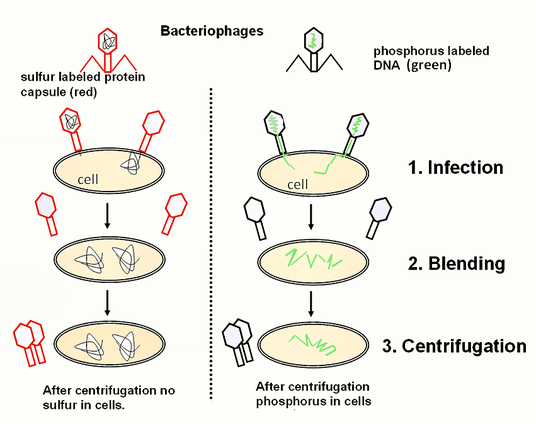
\includegraphics[width=0.6\columnwidth]{images/Martha_Chase_and_Alfred_Hershey_Experiment.png}
   \caption{(\textit{Figura en inglés}) Esquema del experimento de Martha Chase y Alfred Hershey. Más detalles en el texto principal. Fuente \cite{wiki:Alfred_Hershey_and_Martha_Chase_Experiment}}
   \label{fig:Martha_and_Hershey_Experiment}
\end{figure}

% 4
En 1944, ya se había observado que el ADN extraído de una cepa de bacteria podía transferir su virulencia a otra cepa anteriormente inofensiva \cite{averySTUDIESCHEMICALNATURE1944}.
Pero los experimentos decisivos se llevaron a cabo en 1952 por Martha Chase y Alfred Hershey.
En este experimento \cite{hersheyIndependentFunctionsViral1952} los autores emplearon bacteriófagos (virus compuestos solo de ADN y proteínas) para dilucidar qué sustancia penetraba la célula (figura \ref{fig:Martha_and_Hershey_Experiment}).
Resulta que el ADN carece de azufre en su composición, mientras que las proteínas del virus sí presentan este elemento.
Por otro lado, el ADN es rico en fósforo, mientras que las proteínas en cuestión carecían de este.
Esta diferencia permitió marcar ambas sustancias de manera independiente y al infestar las bacterias, solo el fósforo marcado fue detectado su interior.
El resultado era claro, la única sustancia proveniente de los virus que penetraba la célula era el ADN, llevando con ella la información necesaria para producir nuevos bacteriófagos.
 
\begin{figure}[tb]
   \centering
   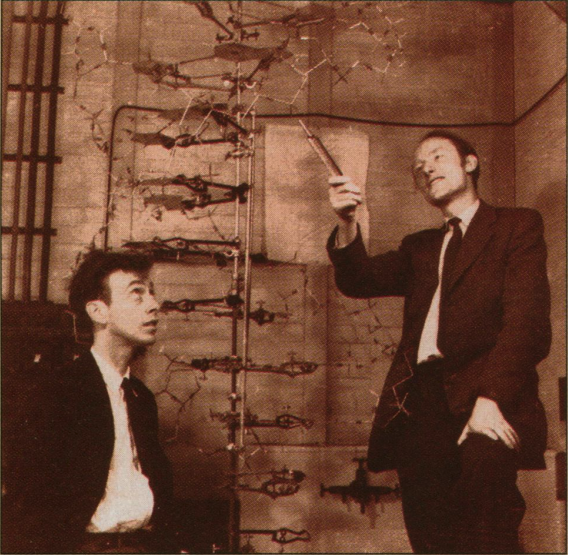
\includegraphics[width=0.6\columnwidth]{images/Watson_and_Crick.png}
   \caption{Watson and Crick frente al modelo de doble hélice. Fuente \cite{hallOldSchoolTies1993}}
   \label{fig:Watson_and_Crick}
\end{figure}
 
% 5
Casi al unísono, en 1953, otro importante descubrimiento fue publicado: la estructura del ADN \cite{watsonMolecularStructureNucleic1953}.
Usando cristalografía de rayos X James Watson and Francis Crick (figura \ref{fig:Watson_and_Crick}) establecieron que el ADN es un polímero con una conformación en doble hélice donde las bases nitrogenadas están apareadas por afinidad química.
Estos resultados sugerían que la información genética estaba codificada en la larga secuencia de esos pares.
Toda la diversidad de la vida ``escrita'' en un mismo lenguaje.
Había nacido la Genética Molecular.

% 5
También de relevante en ese período fue el trabajo de Frederick Sanger, quien publicó en 1951 la secuencia de una de las cadenas de la Insulina \cite{sangerAminoacidSequencePhenylalanyl1951}.
Estos resultados terminaron de imponer la teoría de que las proteínas son polímeros de aminoácidos con una secuencia lineal definida.
El vínculo entre la estructura de las proteínas y la secuencia de ADN era más evidente que nunca antes.
Comenzaban así a dibujarse los primeros bosetos del dogma central de la Biología Molecular.
